\documentclass{article}

\usepackage[T1]{fontenc}
\usepackage[polish]{babel}
\usepackage[utf8]{inputenc}
\usepackage{amsmath}
\usepackage{hyperref}
\usepackage{tablefootnote}
\usepackage{graphicx}
\usepackage{siunitx}
\usepackage{listings}
\usepackage{xcolor}

\lstset{frame=tb,
  language=Python,
  aboveskip=3mm,
  belowskip=3mm,
  showstringspaces=false,
  columns=flexible,
  basicstyle={\small\ttfamily},
  numbers=none,
  numberstyle=\tiny\color{gray},
  keywordstyle=\color{blue},
  commentstyle=\color{dkgreen},
  stringstyle=\color{green},
  breaklines=true,
  breakatwhitespace=true,
  tabsize=3
}

\graphicspath{ {./media/} }

\begin{document}

\section{Cel ćwiczenia}
Celem ćwiczenia jest pomiar siły elektrodynamicznej (przy pomocy wagi) działającej na odcinek przewodnika z prądem, który został umieszczony w jednorodnym polu magnetycznym. Badana jest zależność tej siły od natężenia prądu płynącego w przewodniku i od indukcji pola magnetycznego. Na podstawie przeprowadzonych pomiarów wyznaczana jest wartość indukcji pola magnetycznego

\section{Wyznaczanie siły działającej na fragment przewodnika}
\subsection{pomierzone dane}

$U$ = 12 V
\begin{center}
\begin{tabular}{ c | c | c}
I [A] & m [g] & F [N] * $10^{-3}$\\
\hline
0,5 & 38,19 & 8,93 $\pm$ 0,00\\
1,0 & 39,08 & 17,67 $\pm$ 0,01\\
1,5 & 39,96 & 26,30 $\pm$ 0,01\\
2,0 & 40,85 & 35,04 $\pm$ 0,02\\
2,5 & 41,60 & 42,4 $\pm$ 0,02\\
3,0 & 42,74 & 53,59 $\pm$ 0,03\\
3,5 & 43,67 & 62,72 $\pm$ 0,03\\ 
4,0 & 44,62 & 72,04 $\pm$ 0,04\\
4,5 & 45,44 & 80,09 $\pm$ 0,04\\
5,0 & 46,39 & 89,41 $\pm$ 0,04\\
\end{tabular}
\end{center}

$U$ = 6 V
\begin{center}
\begin{tabular}{ c | c | c}
I [A] & m [g] & F [N]* $10^{-3}$\\
\hline
0,5 & 37,61  & 3,24 $\pm$ 0,00\\
1,0 & 38,01  & 7,16 $\pm$ 0,00\\
1,5 & 38,38  & 10,80 $\pm$ 0,01\\
2,0 & 38,77  & 14,62 $\pm$ 0,01\\
2,5 & 39,14  & 18,26 $\pm$ 0,01\\
3,0 & 39,52  & 21,99 $\pm$ 0,01\\
3,5 & 39,98  & 26,50 $\pm$ 0,01\\
4,0 & 40,31  & 29,74 $\pm$ 0,02\\
4,5 & 40,74  & 33,96 $\pm$ 0,02\\
5,0 & 41,11  & 37,59 $\pm$ 0,02\\
\end{tabular}
\end{center}

$I$ - prąd płynądy przez ramkę \\
$m$ - masa pozorna ramki przy płynącym przez nią prądzie I \\\\
$m_0$ - masa ramki = 37,28 g\\
$g$ - przyspiespieszenie ziemskie przyjęte dla Gdańska $\approx$ 9,815 [$\frac{m}{s^2}$]

\subsection{wykres zależnoci F= f(I)}
$U$ =12 V\\

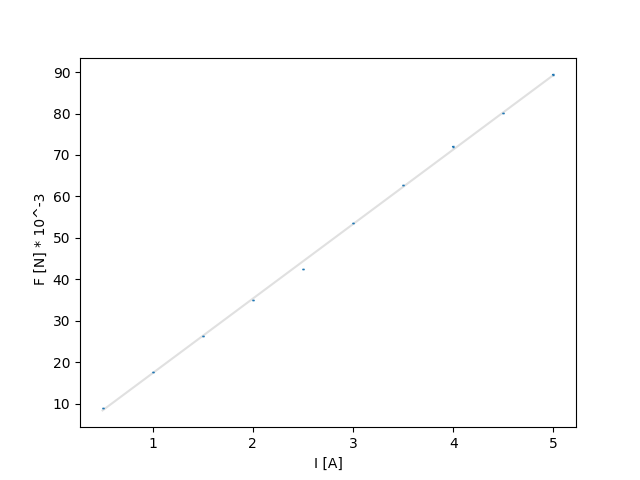
\includegraphics[width=10cm]{F(I)_12V}

$U$ = 6 V\\
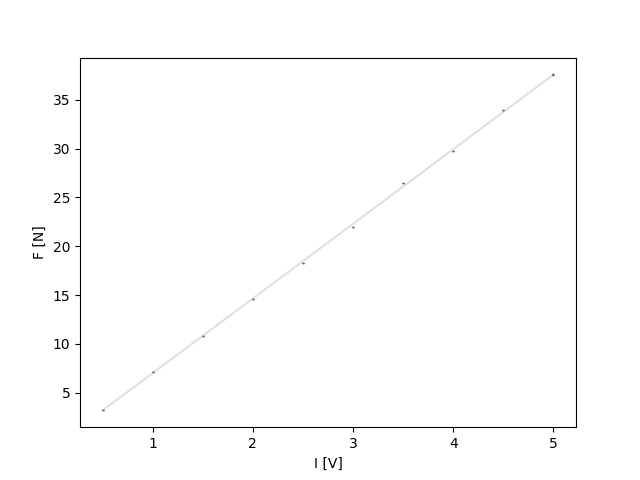
\includegraphics[width=10cm]{F(I)_6V}
\subsection{Niepewności}
Niepewność siły elektrodynamicznej wyznaczamy jako niepewność wielkości złożonej ze wzoru:\\
\begin{gather*}
		\Delta F= |\frac{\partial F}{\partial m}| \Delta m + |\frac{\partial F}{\partial m_0}| \Delta m_0  = (\frac{(m - m_0)g }{m} + \frac{(m - m_0)g }{m_0}) \Delta m
\end{gather*}
gdzie $\Delta m_0 =\Delta m = 0,01$ g
\section{Określenie zależności indukcji magnetycznej elektromagnesu}

\begin{center}
  \begin{tabular}{ c | c | c | c}
  U [V] & I [A] & m [g] & B [T] * $10^{-3}$\\
  \hline
  2 & 0,04 & 37,67 & 956,96 $\pm$ 0,22\\
  4 & 0,2 & 38,96 & 824,46 $\pm$ 0,19\\
  6 & 0,36 & 40,27 & 815,19 $\pm$ 0,19\\
  8 & 0,53 & 41,68 & 814,83 $\pm$ 0,19\\
  10 & 0,7 & 43,11 & 817,45 $\pm$ 0,19\\
  12 & 0,86 & 44,52 & 826,29 $\pm$ 0,19\\
  \end{tabular}
\end{center}

$I$ - natężenie prądu w uzwojeniu elektromagnesu \\
$m$ - masa pozorna ramki przy płynącym przez nią prądzie I \\\\
$m_0$ - masa ramki = 37,28 g\\
$g$ - przyspiespieszenie ziemskie przyjęte dla Gdańska $\approx$ 9,815 [$\frac{m}{s^2}$]

\subsection{Niepewności}
Niepewność indukcji pola magnetycznego wyznaczonego metodą najmniejszych kwadratów wyznaczymy z odpowiednich wzorów  \footnote{\url{https://ftims.pg.edu.pl/documents/10673/20436990/wstep.pdf}}\:

\begin{gather*}
		u_a = \sqrt{\frac{n}{n-2} * \frac{\Sigma y_i^2 - a\Sigma x_iy_i}{n\Sigma x_i^2}} 
\end{gather*}
skąd
\begin{gather*}
		u_B= |\frac{\partial B}{\partial a}| u_a = \frac{g}{L}u_a
\end{gather*}
W przypadku zależności $B(I_m)$ niepewność B wyznaczamy jako niepewność funkcji złożonej zmiennych 
$m, m_0, I$:

\begin{gather*}
		\Delta B = |\frac{\partial B}{\partial m_0}|\Delta m_0 + |\frac{\partial B}{\partial m}|\Delta m + |\frac{\partial B}{\partial I}|\Delta I = \frac{g}{IL}(\Delta m + \Delta m_0 + \frac{m-m_0}{I}\Delta I)
\end{gather*}
gdzie $\Delta m_0 =\Delta m = 0,01$ g oraz $\Delta I = 0,02$ A.

\section{Wartość indukcji magnetycznej w szczelinie elektomagnesu}

a, b = 1.83 37.21
(wyszlo w 1 przykladzie a = 1.82 więc się zgadza)

\section{Użyte wzory}

\subsection{Wyniki}
Przy pierwszych pomiarach (zmienianie prądu płynącego w ramce) chcąc wyznaczyć 
wartość indukcji pola magnetycznego B posłużymy się wzorem:
\begin{gather*}
	F = ILB \\
	(m-m_0)g = ILB \\
	m(I) = \frac{LB}{g}I + m_0
\end{gather*} 
gdzie $m_0$ - masa samej ramki,\\
$m$ - masa pozorna ramki przy płynącym przez nią prądzie I \\
$L=0,1$ m\footnote{\url{https://pg.edu.pl/files/ftims/2021-03/cwiczenieE5.pdf}} - długość odcinka przewodnika oddziałującego z polem magnetycznym. \\
Korzystając z metody najmniejszych kwadratów otrzymamy wspł.  kierunkowy prostej
\begin{gather*}
	a = \frac{LB}{g} \rightarrow B = \frac{ag}{L}
\end{gather*}
W następym pomiarze (zmiana prądu płynącego przez uzwojenie elektromagnesu) skorzystamy z zależności
\begin{gather*}
	B = \frac{(m-m_0)g}{IL}
\end{gather*}
przy określeniu zależności $B(I_m)$, gdzie $I_m$ - natężenie prądu w uzwojeniu elektromagnesu.




\end{document}